\documentclass[pdf]{beamer} 
2 \usepackage[utf8]{inputenc} 
3 \usepackage{graphicx} 
4 \usepackage[squaren, Gray]{SIunits} 
5 \usepackage{amsmath}  
6 \usepackage{tabularx} 
7 
 
8 \usetheme{warsaw} 
9 \mode<presentation>{} 
10 
 
11 \title{Physique} 
12 \subtitle{APP 2 : Propagation des ondes électromagnétiques} 
13 \author{Groupe 1243} 
14 
 
15 \begin{document} 
16 
 
17 \begin{frame} 
18 	\titlepage 
19 \end{frame} 
20 
 
21 \begin{frame}{Réponses aux questions du texte} 
22 \textbf{Quelle est la quantité moyenne d'énergie provenant du rayonnement du soleil 
23 arrivant sur la surface de la terre?} 
24 D'après \textsc{Rosner} et \textsc{Robert} dans \textit{MacMillan Encyclopedia of Physics, vol. 4}, cette énergie  
25 moyenne, appelée constante solaire vaut approximativement $\unit{1.4}{\kilo\watt\per\meter\squared}$. 
26 
 
27 % On devait calculer cette valeur ou bien la trouver par une recherche? 
28 
 
29 \textbf{Comment expliquer l'existence des saisons?} 
30 L'axe de rotation de la terre est penché par rapport à son plan orbital, et c'est ce qui cause les saisons 
31 sur terre. Selon l'inclinaison de la terre, les rayonnements de soleil s'étaleront plus ou moins 
32 sur différentes zones de la terre. La densité d'énergie variera alors aussi. 
33 \end{frame} 
34 
 
35 \begin{frame}{Comment expliquer l'existence des saisons?} 
36 	\begin{figure}[ht!] 
37     \centering 
38     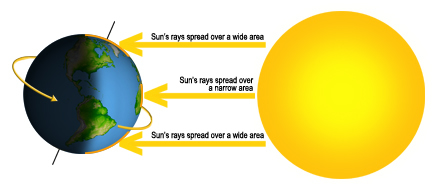
\includegraphics[scale=0.75]{whyseasons.jpg} 
39 		\caption{Inclinaison de la terre par rapport au soleil. (Source : http://www.lpi.usra.edu/)} 
40 	\end{figure} 
41 \end{frame} 
42 
 
43 \begin{frame}{Réponses aux questions du texte} 
44 \textbf{Comment distinguer/classer les ondes électromagnétiques?} 
45 On peut distinguer differents types d'ondes électromagnétiques selon leur fréquence 
46 et leur longueur d'onde (exemples : microonde, infrarouge, ultraviolet, rayons X,  
47 rayons gammas, etc). 
48 \textbf{Combien de temps met la lumière du soleil pour nous arriver?} 
49 Etant donné la vitesse de la lumière $c = \unit{3 \cdot 10^8}{\meter\per\second}$ et la 
50 distance terre soleil $d_{t-s} = \unit{149600000}{\kilo\meter}$, on trouve $t = \unit{498.66}{\second} 
51 = \unit{8.31}{\minute}$. \\ 
52 \textbf{Même question pour le signal envoyé par un satellite géostationnaire?} 
53 Cette fois, $d_{t-sat} = \unit{35786}{\kilo\meter}$ (pour un satellite géostationnaire, selon 
54 Wikipédia). On a donc $t = \unit{0.11}{\second}$. 
55 \end{frame} 
56 
 
57 \begin{frame}{Propagation d'un champ magnétique et d'un champ électrique sans support} 
58 	Sans support $\Rightarrow \rho = 0$ et $\vec{J} = \vec{0}$. 
59 	La loi de \textsc{Faraday} et la loi d'\textsc{Ampère} peuvent donc se réecrire : 
60 	 
61 	$$ 
62 	\left\{ 
63 		\begin{array}{rl} 
64 			\vec{\nabla} \times \vec{E} &= -\frac{\delta \vec{B}}{\delta t}\\ 
65 			\vec{\nabla} \times \vec{B} &= \mu_0 \epsilon_0 \frac{\delta \vec{E}}{\delta t} 
66 		\end{array} 
67 	\right 
68 	$$ 
69 	 
70 	On voit donc qu'une variation spatiale de $\vec{E}$ entraine une variation temporelle de $\vec{B}$ 
71 	et qu'une variation spatiale de $\vec{B}$ entraine une variation temporelle de $\vec{E}$. 
72 	On remarque donc très facilement que le champ magnétique et le champ électrique sont dépendants l'un de l'autre. 
73 	 
74 	% A expliquer plus en profondeur. 
75 \end{frame} 
76 
 
77 \begin{frame}{Temps de propagation dans un diélectrique} 
78 	En sachant 
79 	que l'indice de réfraction $n$ du verre est approximativement de $1.6$ (Source : List of refractive indices sur Wikipedia) 
80 	, on peut calculer la vitesse de propagation de la lumière dans le verre. 
81 	 
82 	$$n = \frac{c}{v} \Rightarrow v = \frac{c}{1.6} = \unit{1.875 \cdot 10^8}{\meter\per\second}$$ 
83 	 
84 	En reprenant la distance terre-soleil $d = \unit{149600000}{\kilo\meter}$, on a alors $t = \unit{797.86}{\second} = 
85 	\unit{13.29}{\minute}$. 
86 \end{frame} 
87 
 
88 \begin{frame}{Seconde étape} 
89 	\textbf{Forme générale d'une fonction qui se déplace à une vitesse $v$ dans la direction $x$ :} 
90 	$$u(x, t) = f(x - vt)$$ 
91 	 
92 	\textbf{Cas sinusoidal :} 
93 	$$u(x, t) = A \cos{(kx - \omega t)}$$ 
94 \end{frame} 
95 
 
96 \begin{frame}{Seconde étape} 
97 	\textbf{Orientations vectorielles des champs électrique et magnétique et direction de propagation :} 
98 		$\vec{B}$ et $\vec{E}$ sont perpendiculaires et la direction de propagation est donnée par $\vec{E} \times 
99 		\vec{B}$. 
100 		\begin{figure}[ht!] 
101 			\centering 
102 			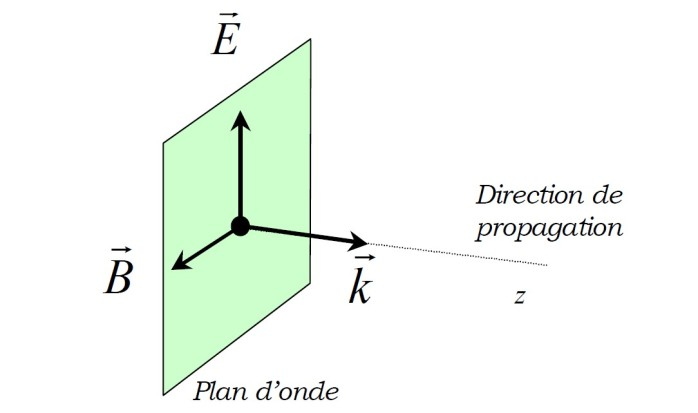
\includegraphics[scale=0.4]{direction-be.jpg} 
103 			\caption{(Source : http://res-nlp.univ-lemans.fr/)} 
104 		\end{figure} 
105 \end{frame} 
106 
 
107 \begin{frame}{Propagation du signal en fonction du temps et de l'espace parcouru} 
108 	\begin{figure}[ht!] 
109     \centering 
110     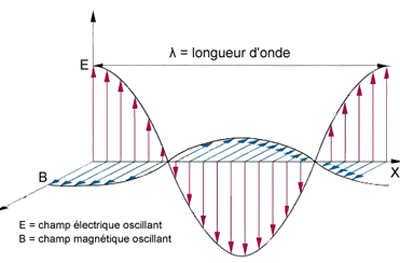
\includegraphics[scale=0.7]{signal.png} 
111 		\caption{(Source : sweetrandomscience)} 
112 	\end{figure} 
113 \end{frame} 
114 
 
115 \begin{frame}{Comparaisons de différents types d'ondes électromagnétiques} 
116 		% 
117 	\begin{center} 
118 		\begin{tabular}{c|c|c|c} 
119 											& Bande de fréquences		& Longueurs d'ondes 			& Nombre d'ondes							 \\ 
120 			\hline 
121 			Rayons X				& $\unit{3 \cdot 10^{16}}{\hertz}$ à $\unit{3 \cdot 10^{19}}{\hertz}$		 
122 											& 								 
123 											& $\unit{10^{-11}}{\meter}$ à $\unit{10^{-8}{\meter}$ \\ 
124 			\hline 				& $\unit{4 \cdot 10^{14}}{\hertz}$ à $\unit{8 \cdot 10^{14}}{\hertz}$ 
125 			Lumière visibe	& 											 
126 											& 												 
127 											& $\unit{7,8\cdot10^{-7}}{\meter}$ à $\unit{3,8 \cdot 10^{-7}{\meter}$ \\ 
128 			\hline 
129 			Ondes radio				& $\unit{1}{\hertz}$ à $\unit{1 \cdot 10^{9}}{\hertz}$											 
130 											& 												 
131 											& $\unit{1000}{\meter}$ à $\unit{0,3 {\meter}$\\ 
132 			\hline 
133 			Hyperfréquence				& $\unit{1 \cdot 10{9}}{\hertz}$ à $\unit{3 \cdot 10^{11}}{\hertz}$											 
134 											& 												 
135 											& $\unit{0.3}{\meter}$ à $\unit{1 \cdot 10^{-3} {\meter}$\\ \\ 
136 			\hline 
137 			Infrarouge				& $\unit{3 \cdot 10{11}}{\hertz}$ à $\unit{4 \cdot 10^{14}}{\hertz}$											 
138 											& 												 
139 											& $\unit{1 \cdot 10^{-3}}{\meter}$ à $\unit{7,8 \cdot 10^{-7} {\meter}$ \\ 
140 		\end{tabular} 
141 	\end{center} 
142 \end{frame} 
143 
 
144 \end{document} 


\begin{frame}{Seconde étape}
	\textbf{Orientations vectorielles des champs électrique et magnétique et direction de propagation :}
		$\vec{B}$ et $\vec{E}$ sont perpendiculaires et la direction de propagation est donnée par $\vec{E} \times
		\vec{B}$.
		\begin{figure}[ht!]
			\centering
			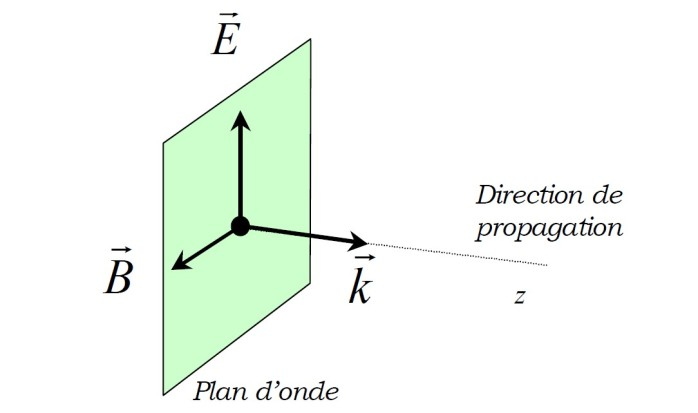
\includegraphics[scale=0.4]{direction-be.jpg}
			\caption{(Source : http://res-nlp.univ-lemans.fr/)}
		\end{figure}
\end{frame}

\begin{frame}{Propagation du signal en fonction du temps et de l'espace parcouru}
	\begin{figure}[ht!]
    \centering
    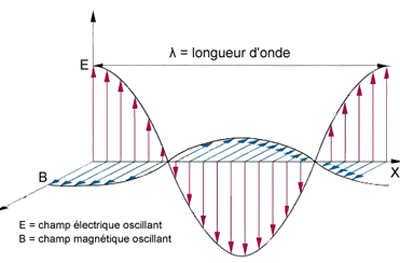
\includegraphics[scale=0.7]{signal.png}
		\caption{(Source : sweetrandomscience)}
	\end{figure}
\end{frame}

%\begin{frame}{Comparaisons de différents types d'ondes électromagnétiques}
		%
	%\begin{center}
		%\begin{tabular}{c|c|c|c}
											%& Bande de fréquences		& Longueurs d'ondes 			& Nombre d'ondes							 \\
			%\hline
			%Rayons X				& $\unit{3 \cdot 10^{16}}{\hertz}$ à $\unit{3 \cdot 10^{19}}{\hertz}$		
											%& 								
											%& $\unit{10^{-11}}{\meter}$ à $\unit{10^{-8}{\meter}$ \\
			%\hline
			%Lumière visibe	& 											
											%& 												
											%&  \\
			%\hline
			%Ondes radio			& 											
											%& 												
											%&  \\
			%\hline
			%Hyperfréquence	& 											
											%& 												
											%&  \\
			%\hline
			%Infrarouge			& 											
											%& 												
											%&  \\
		%\end{tabular}
	%\end{center}
%\end{frame}

\end{document}
